\noindent{\Huge\scshape Х}{\LARGE\scshape имия}\\
\rule[0.5\baselineskip]{\textwidth}{1pt}

\vspace{0\baselineskip}

\subsection*{Задание 10.}
Жук-бомбардир получил своё название благодаря своеобразному защитному механизму. Он способен громко выстреливать из задней части%
\setlength{\intextsep}{0.2pt} 
\setlength\columnsep{15.2pt}
\begin{wrapfigure}[10]{l}{4.4cm}
{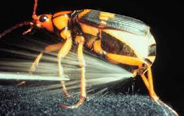
\includegraphics[width=4.6cm]{images/10-1.png}}
\caption{Стреляющий австралийский \textit{Pheropsophus verticalis}}\label{fig:chim1}
\end{wrapfigure}
брюшка токсичной саморазогревающейся смесью (рис.~\ref{fig:chim1}). Бензохинон, ключевой компонент этой смеси, раздражает глаза и дыхательные системы у позвоночных.

«Пушкой» жука-бомбардира является пара двухкамерных пигидиальных желёз (рис.~\ref{fig:image2}). В \textbf{резервуаре} вырабатывается водная смесь, состоящая из перекиси водорода, метилгидрохинона и других вспомогательных веществ. В \textbf{реакторе} постоянно присутствуют ферменты каталаза и пероксидаза. На конце железы находится твердое \textbf{выходное отверстие}, служащее «дулом» для прицельной наводки при стрельбе.

\mbox{\textbf{Вопрос 1}.} Нарисуй структуры метилгидрохинона и метил-\textit{пара}-бен\-зо\-хи\-но\-на.\vspace{1ex}
    
Из \textbf{резервуара} в \textbf{реакционную камеру} попадает капля водного раствора, содержащая $25\,\%$ пероксида водорода и $10\,\%$ метилгидрохинона. Далее происходят сразу три химических процесса:
\begin{list}{\Asbuk{nnn})}{\usecounter{nnn}\leftmargin=6mm \labelwidth=5mm \topsep=0mm \labelsep=2mm \itemsep=0pt \parsep=0mm \itemindent=-1pt}
\item метилгидрохинон превращается в соответствующий метил-\textit{пара}-бен\-зо\-хи\-нон с отщеплением водорода. Реакция катализируется пероксидазой и проходит с поглощением 177~кДж/моль теплоты,
\item каталаза катализирует разложение пероксида водорода с образованием кислорода и воды. При этой реакции выделяется 94,5~кДж/моль теплоты,
\item водород и кислород реагируют с образованием воды и выделением 286~кДж/моль теплоты.
\end{list}

\setlength{\columnsep}{5.2pt}
\begin{wrapfigure}[13]{l}{4.7cm}{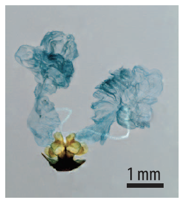
\includegraphics[width=4.6cm]{images/10-2.png}}\caption{Строение пи\-ги\-даль\-ных желёз жука-бом\-бар\-ди\-ра}
\label{fig:image2}\end{wrapfigure}
\mbox{\textbf{Вопрос 2}.} Напиши термохимические уравнения реакций А-В.
\vspace{1ex}
 	
\mbox{\textbf{Вопрос 3}.} Напиши суммарное термохимическое уравнение, описывающее все три процесса.\vspace{1ex}
    
\mbox{\textbf{Вопрос 4}.} По рентгенографическим данным, диаметр капли раствора составляет $0{,}2$~мм. Определи объём капли и количества пероксида водорода и метилгидрохинона, которые в ней содержатся.\vspace{1ex}
    
\mbox{\textbf{Вопрос 5}.} Определи температуру нагрева капли в результате обсуждаемых химических превращений ($T_{\text{жука}} = 36{,}6\,^\circ\mathsf{C}$), если бы количество метилгидрохинона равнялось количеству пероксида водорода.\vspace{1ex} 	
    
\setlength{\intextsep}{0.2pt} 
\setlength{\columnsep}{15.2pt}
\begin{wrapfigure}[11]{r}{4.4cm}{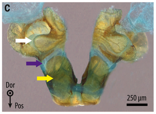
\includegraphics[width=4.6cm]{images/10-3.png}}\caption{Строение «спускового механизма» пигидальной железы}\label{fig:image3}
\end{wrapfigure}
Оставшийся пероксид водорода расходуется на то, чтобы создать избыточное давление в реакционной камере жука для выстрела (рис.~\ref{fig:image3}). Жук испускает из своего анального отверстия смесь продуктов вышеуказанных реакций ($T_{\text{выстрела}} = 100\,^\circ$) в импульсном режиме с частотой $1000$~Гц. Известно, что движущей силой этого процесса является избыточное давление в железе, а не мышечные сокращения.\vspace{1ex}

\mbox{\textbf{Вопрос 6}.} Оцени величину критического давления на выходное \textbf{пигидиальное отверстие}, при котором происходит выстрел. Считай, что скорость реакции достаточна для того, чтобы за период между выстрелами всё вступающее в реакцию вещество прореагировало, а реакционная камера представляет собой сферу радиуса $0{,}25$~мм.
 	
\subsection*{Задание 11.}
В насыщенный водный раствор $\mathsf{FeCl}_2$ массой $80$~г внесли $20$~г безводной соли. При нагревании весь осадок растворился и раствор охладили до исходной температуры. При этом выпало $48{,}6$~г осадка кристаллогидрата. Установи формулу кристаллогидрата, если известно, что насыщенный раствор содержит $38{,}5\,\%$ безводной соли. 

%======================= cut off ==============
\iffalse\begin{itemize}
\item В исходном растворе $80\times 0{,}385 = 30{,}8$~г. безводной соли и $80 - 30,8 = 49,2$~г. воды; $80+20 = 100$~г. — масса раствора после растворения безводной соли.
\item Масса раствора после выпадения кристаллогидрата: $100 - 48,6= 51,4$~г. — масса насыщенного раствора исходного состава. 
\item В нём соли $51,4\times0,385 = 19,789$~г., а воды $51,4 - 19,789  = 31,611$~г..
\item Воды в кристаллогидрате: $49,2 - 31,611 = 17,598$~г.
\item Масса безводной соли в кристаллогидрате: $48,6 - 17,598  = 31,011$~г.
\item Отношение в кристаллогидрате ``соль\,:\,вода'': $31{,}011/127 \div 17{,}598/18 = 1\div 4$.
\item Формула кристаллогидрата — $\mathsf{FeCl}_2*4H_2O$.
\end{itemize}\fi
%======================== end of cut-off===========

\subsection*{Задание 12.}
Четвёртого мая $1958$ года в одной лаборатории оставили запаянную ампулу объёмом $100$ мл с $^{63}Ni(CO)_4$ массой $5$~г. При радиоактивном $\beta$-распаде никеля-$63$ карбонил разлагается на чистый металл и угарный газ, с периодом полураспада $100,1$ лет. Зная, что ампула была запаяна в атмосфере азота при н.\,у., укажи, во сколько раз изменилось давление в ней на сегодняшний день, а также массу и состав осадка. (Укажи дату решения, объёмом негазообразных веществ пренебречь.)

%=========================== cut-off ====================
\iffalse\begin{itemize}
\item $No=5/175\times 6.023\times10(23)=1.72\times10(22)$
\item $N=No\times2^{-(t/T)}=1.72\times10(22)\times0.66=1.13\times10(22)$
\item $n(Ni(CO)_4)$ разложившегося — $0.0188$~моль
\item $n(CO)=0.075$~моль, $n(N2)= 0.045$~моль.
\end{itemize}\fi
%====================== end of cut-off ==============